\documentclass[aspectratio=169]{beamer}
\usepackage[utf8]{inputenc}
\usepackage[T1]{fontenc}
\usepackage{graphicx}
\usepackage{booktabs}
\usepackage{csquotes}
\usepackage{hyperref}
\usepackage{caption}
\usepackage{subcaption}
\usepackage{amsmath}
\usepackage{amssymb}

\usepackage[backend=biber,style=authoryear]{biblatex}
\usepackage{url}

\setbeamertemplate{navigation symbols}{}
\addbibresource{citations.bib}

\AtBeginSection[]{
    \begin{frame}[plain]
        \sectionpage
    \end{frame}
}

\usetheme{Madrid}
\usecolortheme{whale}
\setbeamertemplate{caption}[numbered]

\title[Integrating logical constraints in OCGNN for AD]{Integrating Logical Constraints \\in One-Class Graph Neural Networks for Anomaly Detection}
\subtitle{Final Presentation}
\author[A. Romanenko]{Anastasiia Romanenko}
\institute[TU Dortmund]{Technische Universit\"at Dortmund \\ Fakult\"at Statistik}
\date{\today}

\begin{document}

\begin{frame}
  \titlepage
  \vspace{1cm}
  \centering
  \small
  Supervisors: Prof.\ Dr.\ Emmanuel M\"uller, Tim Katzke
\end{frame}

\begin{frame}{Contents}
  \tableofcontents
\end{frame}

\section{Problem Statement}

\begin{frame}{Importance of Anomaly Detection on Graph Data}
    An anomaly is an unusual or unexpected pattern in data. Detecting anomalies is important for identifying unknown threats and irregular behavior in complex systems.

    \begin{figure}[htpb]
        \centering
        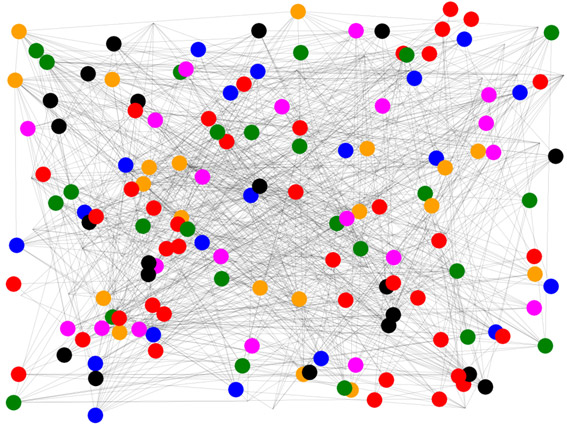
\includegraphics[width=7cm]{images/graph_picture.jpg}
    \end{figure}
\end{frame}

\begin{frame}{Motivation of Constraints Driven Graph AD}
    In many real-world applications we have prior knowledge about data, which can be formulated as logical rules

    \begin{itemize}
        \item If $\texttt{person\_height} > 200\,\text{cm}$ $\rightarrow$ anomaly
        \item If a financial transaction graph contains a forbidden cycle pattern $\rightarrow$ anomaly
        \item If a molecular graph violates valence constraints $\rightarrow$ anomaly
    \end{itemize}
    \vspace{0.4cm}
    \textbf{Classical One-Class Graph Neural Networks:}
    \begin{itemize}
        \item learn only from data
        \item do not explicitly learn logical rules
        \item may learn representations that violate known knowledge
    \end{itemize}
\end{frame}

\section{Background}

\begin{frame}{Anomalies on Graph Data}
    \begin{figure}[htpb]
        \centering
        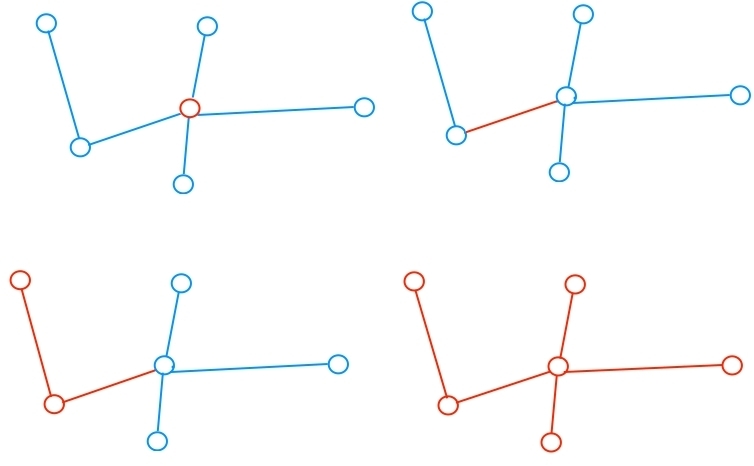
\includegraphics[width=10cm]{images/anomalies.jpg}
        \caption{Kinds of anomalies on graph data}
    \end{figure}
\end{frame}

\begin{frame}{Previous One-Class Graph Methods}
    \textbf{Common assumptions:}
    \begin{itemize}
        \item Access to a large set of normal graph data only
        \item Learn a graph embedding $f_\theta(G) \in \mathbb{R}^d$
        \item Model ``normality'' as a compact region in the embedding space
    \end{itemize}

    \textbf{Typical objective (hypersphere learning):}
    \[
    \min_{\theta} \sum_{i}
    \left\| f_\theta(G_i) - c \right\|^2
    \]
    where $c$ denotes the center of normal data.
\end{frame}

\begin{frame}{OCGNN -- Structure and Forward Pass}
    \begin{figure}[htpb]
        \centering
        
\includegraphics[width=14cm]{images/ocgin.pdf}
        \caption{Structure of OCGIN \footcite{ocgin}}
    \end{figure}

    \vspace{-0.3cm}
    \begin{columns}
        \column{0.5\textwidth}
        \textbf{GIN Layer:}
        \[
        h_v^{(k+1)} = \text{MLP}^{(k)}\bigl((1+\epsilon)h_v^{(k)} + \sum_{u \in \mathcal{N}(v)} h_u^{(k)}\bigr)
        \]
        \column{0.5\textwidth}
        \textbf{Deep SVDD Loss:}
        \[
        \mathcal{L} = \frac{1}{n} \sum_{i=1}^{n} \| z_i - c \|^2
        \]
    \end{columns}
\end{frame}

\begin{frame}{Existing Methods with Logical Constraints}
    \textbf{1) Constraints as Semantic Loss \footcite{xu2018semanticlossfunctiondeep}}
    \begin{itemize}
      \item Logical rules encoded as differentiable loss terms
      \item Minimize both data loss and constraint loss
    \end{itemize}

    \textbf{2) Fuzzy Logic in Loss \footcite{Badreddine_2022}}
    \begin{itemize}
      \item Logical rules relaxed by applying continuous functions
    \end{itemize}

    \textbf{3) Constraint-aware Architectures \footcite{yang2023injectinglogicalconstraintsneural}}
    \begin{itemize}
      \item Logical rules compiled into network structure or output layer
    \end{itemize}
\end{frame}

\begin{frame}{Assumptions and Empirical Results}
    \textbf{Common Assumptions}
    \begin{itemize}
      \item Domain knowledge is available in the form of logical rules
      \item Constraints can be formulated as differentiable terms
    \end{itemize}

    \textbf{Empirical Benefits}\footcite{Giunchiglia_2022}, \footcite{stoian2024realisticsyntheticdataconstraining}
    \begin{itemize}
      \item Improved performance
      \item Models learn from less data
      \item Increased interpretability through semantic rule satisfaction
    \end{itemize}
\end{frame}

\section{Methodology}

\begin{frame}{Why Are Graph AD Datasets Uncommon?}
    \textbf{Problem with Collecting Graph AD Datasets:}
    \begin{itemize}
        \item Anomalies are rare, diverse, and unknown (typically $< 5\%$ of data)
        \item Difficult to collect and label
    \end{itemize}

    \textbf{Common Solution: Pseudo-Labels}
    \begin{itemize}
        \item Use labeled graph datasets where one class is treated as normal
        \item Majority class = ``normal'', minority class = ``anomaly''
    \end{itemize}
\end{frame}

\begin{frame}{Constraint Generation from Decision Trees}
    \textbf{Problem:} Domain experts not always available to define rules.

    \textbf{Solution: Automatically generate constraints from decision trees.}

    \begin{enumerate}
        \item Augment node features with structural descriptors:
        \begin{itemize}
            \item Raw node features $\mathbf{x}_v$
            \item Node degree $\deg(v)$
            \item Local clustering coefficient $\text{CC}(v)$
        \end{itemize}
        \item Train a decision tree on (pseudo-)labeled data
        \item Extract logical rules from root-to-leaf paths:
        \[
        r_j: \bigwedge_{\ell=1}^{L} \bigl( x_{f_\ell} \bowtie_\ell \theta_\ell \bigr) \implies \hat{y}_j
        \]
    \end{enumerate}
\end{frame}

\begin{frame}[fragile]{Example: Constraint JSON}
    \begin{small}
    \begin{verbatim}
{
  "constraints": [
    {
      "conditions": [
        {"feature_index": 1263, "op": "<=", "threshold": 0.0},
        {"feature_index": 205, "op": "<=", "threshold": 0.0}
      ],
      "predicted_class": 1,
      "meta": {"depth": 2, "y_label_number": "98 v.s. 243"}
    },
    ...
  ],
  "additional_attributes": {
    "0:1433": "node_features",
    "1433": "node_degree",
    "1434": "clustering_coefficient"
  }
}
    \end{verbatim}
    \end{small}
\end{frame}

\begin{frame}{Differentiable Constraint Evaluation: Fuzzy Logic}
    \begin{columns}
        \column{0.6\textwidth}
        \textbf{Pipeline:}
        \begin{enumerate}
            \item \textbf{Feature Extraction:} Combine original + derived features
            \item \textbf{Rule Evaluation:} For each anomaly rule:
            \begin{itemize}
                \item Evaluate conditions using soft logic
                \item Combine with soft AND (product t-norm)
            \end{itemize}
            \item \textbf{Combine Rules:} Soft OR over all rules
        \end{enumerate}

        \vspace{0.2cm}
        Output: scalar violation score $L_c \in [0,1]$

        \column{0.4\textwidth}
        \textbf{Comparison operators:}
        \begin{itemize}
            \item $x \leq t \rightarrow \sigma(\gamma \cdot (t - x))$
            \item $x > t \rightarrow \sigma(\gamma \cdot (x - t))$
        \end{itemize}

        \textbf{Logic gates:}
        \begin{itemize}
            \item $A \land B \rightarrow \prod_i A_i$
            \item $A \lor B \rightarrow 1 - \prod_i (1 - A_i)$
        \end{itemize}
    \end{columns}
\end{frame}

\begin{frame}{Differentiable Constraint Evaluation: Distance-Based}
    \textbf{Alternative approach:} signed margin scoring to rule boundaries.

    \begin{itemize}
        \item Rules split into $\mathcal{R}_{\text{norm}}$ and $\mathcal{R}_{\text{anom}}$
        \item For each condition: margin $d_c(x) = |x_f - \theta|$
        \item Rule margin: $d(x, r) = \min_{c \in r} d_c(x)$
    \end{itemize}

    \textbf{Three regions:}
    \begin{enumerate}
        \item \textbf{Normal region:} satisfies a normality rule $\rightarrow$ negative score
        \item \textbf{Anomaly region:} satisfies an anomaly rule $\rightarrow$ positive score
        \item \textbf{Grey zone:} satisfies neither $\rightarrow$ linear group distance
    \end{enumerate}

    \vspace{0.2cm}
    Final score: $L_c(x) = \lambda \cdot \sigma(\text{score}(x))$
\end{frame}

\begin{frame}{Loss Integration Strategies}
    Base loss (Deep SVDD):
    \[
    \mathcal{L}_{\text{SVDD}} = \frac{1}{N} \sum_{i=1}^{N} \| z_i - c \|^2
    \]

    \textbf{Variant 1 -- Additive:}
    \[
    \mathcal{L}_{\text{total}} = \frac{1}{N}\sum \|z_i - c\|^2 + \frac{1}{N}\sum L_c^{(i)}
    \]

    \textbf{Variant 2 -- Weighting:}
    \[
    \mathcal{L}_{\text{total}} = \frac{1}{N}\sum \bigl( \|z_i - c\|^2 \cdot (1 + L_c^{(i)}) \bigr)
    \]

    \textbf{Variant 3 -- Suppression:}
    \[
    \mathcal{L}_{\text{total}} = \frac{1}{N}\sum \bigl( \|z_i - c\|^2 \cdot (1 - L_c^{(i)}) \bigr)
    \]
\end{frame}

\begin{frame}{Loss-Only vs.\ Constraint-Aware Inference}
    \textbf{Loss-Only:}
    \begin{itemize}
        \item Constraints used exclusively during training
        \item Anomaly score at inference: $a_i = \| z_i - c \|^2$
        \item Constraints serve as regularisation mechanism
    \end{itemize}

    \textbf{Constraint-Aware Inference:}
    \begin{itemize}
        \item Constraints also applied at inference time
        \item Modified anomaly scores:
        \begin{align*}
            a_i &= \| z_i - c \|^2 + L_c^{(i)} \quad &&\text{(additive)} \\
            a_i &= \| z_i - c \|^2 \cdot (1 + L_c^{(i)}) \quad &&\text{(weighting)}
        \end{align*}
        \item Requires constraints at test time
    \end{itemize}

    $\Rightarrow$ 6 model variants total: 3 loss $\times$ 2 inference paradigms
\end{frame}

\section{Experimental Results}

\begin{frame}{Experimental Setup: Datasets}
    \textbf{15 datasets} across multiple domains:

    \begin{columns}
        \column{0.5\textwidth}
        \textbf{Node-Level (8):}
        \begin{itemize}
            \item \textbf{Planetoid:} Cora, CiteSeer, PubMed
            \item \textbf{Coauthor:} CS
            \item \textbf{Amazon:} Photo
            \item \textbf{WebKB:} Texas, Cornell, Wisconsin
        \end{itemize}

        \column{0.5\textwidth}
        \textbf{Graph-Level (7):}
        \begin{itemize}
            \item \textbf{Bioinformatics:} MUTAG, AIDS, DHFR, ENZYMES, PROTEINS
            \item \textbf{Computer Vision:} COIL-RAG, MSRC\_21
        \end{itemize}
    \end{columns}

    \vspace{0.3cm}
    \textbf{Total: 27,261 individual trials}
\end{frame}

\begin{frame}{Hyperparameter Search Space}
    \begin{table}[h]
    \centering
    \small
    \begin{tabular}{lll}
    \toprule
    Category & Hyperparameter & Values \\
    \midrule
    \multirow{2}{*}{Baseline OCGIN}
    & Hidden dimension & $\{4,8,16,32,64,128,256,512\}$ \\
    & GNN layers & $\{2,3,4,5\}$ \\
    \midrule
    \multirow{4}{*}{Constraint-specific}
    & Scaling $\lambda$ & $\{1,0.5,0.1,0.01,0.001\}$ \\
    & Handler & \{fuzzy logic, distance-based\} \\
    & Integration & \{additive, weighting, suppression\} \\
    & Type & \{training-only, inference-time\} \\
    \bottomrule
    \end{tabular}
    \end{table}

    \textbf{Fixed:} lr = $10^{-3}$, 50 epochs, batch size 32, tree depth 3
\end{frame}

\begin{frame}{Overall Model Comparison}
    \begin{figure}[htpb]
        \centering
        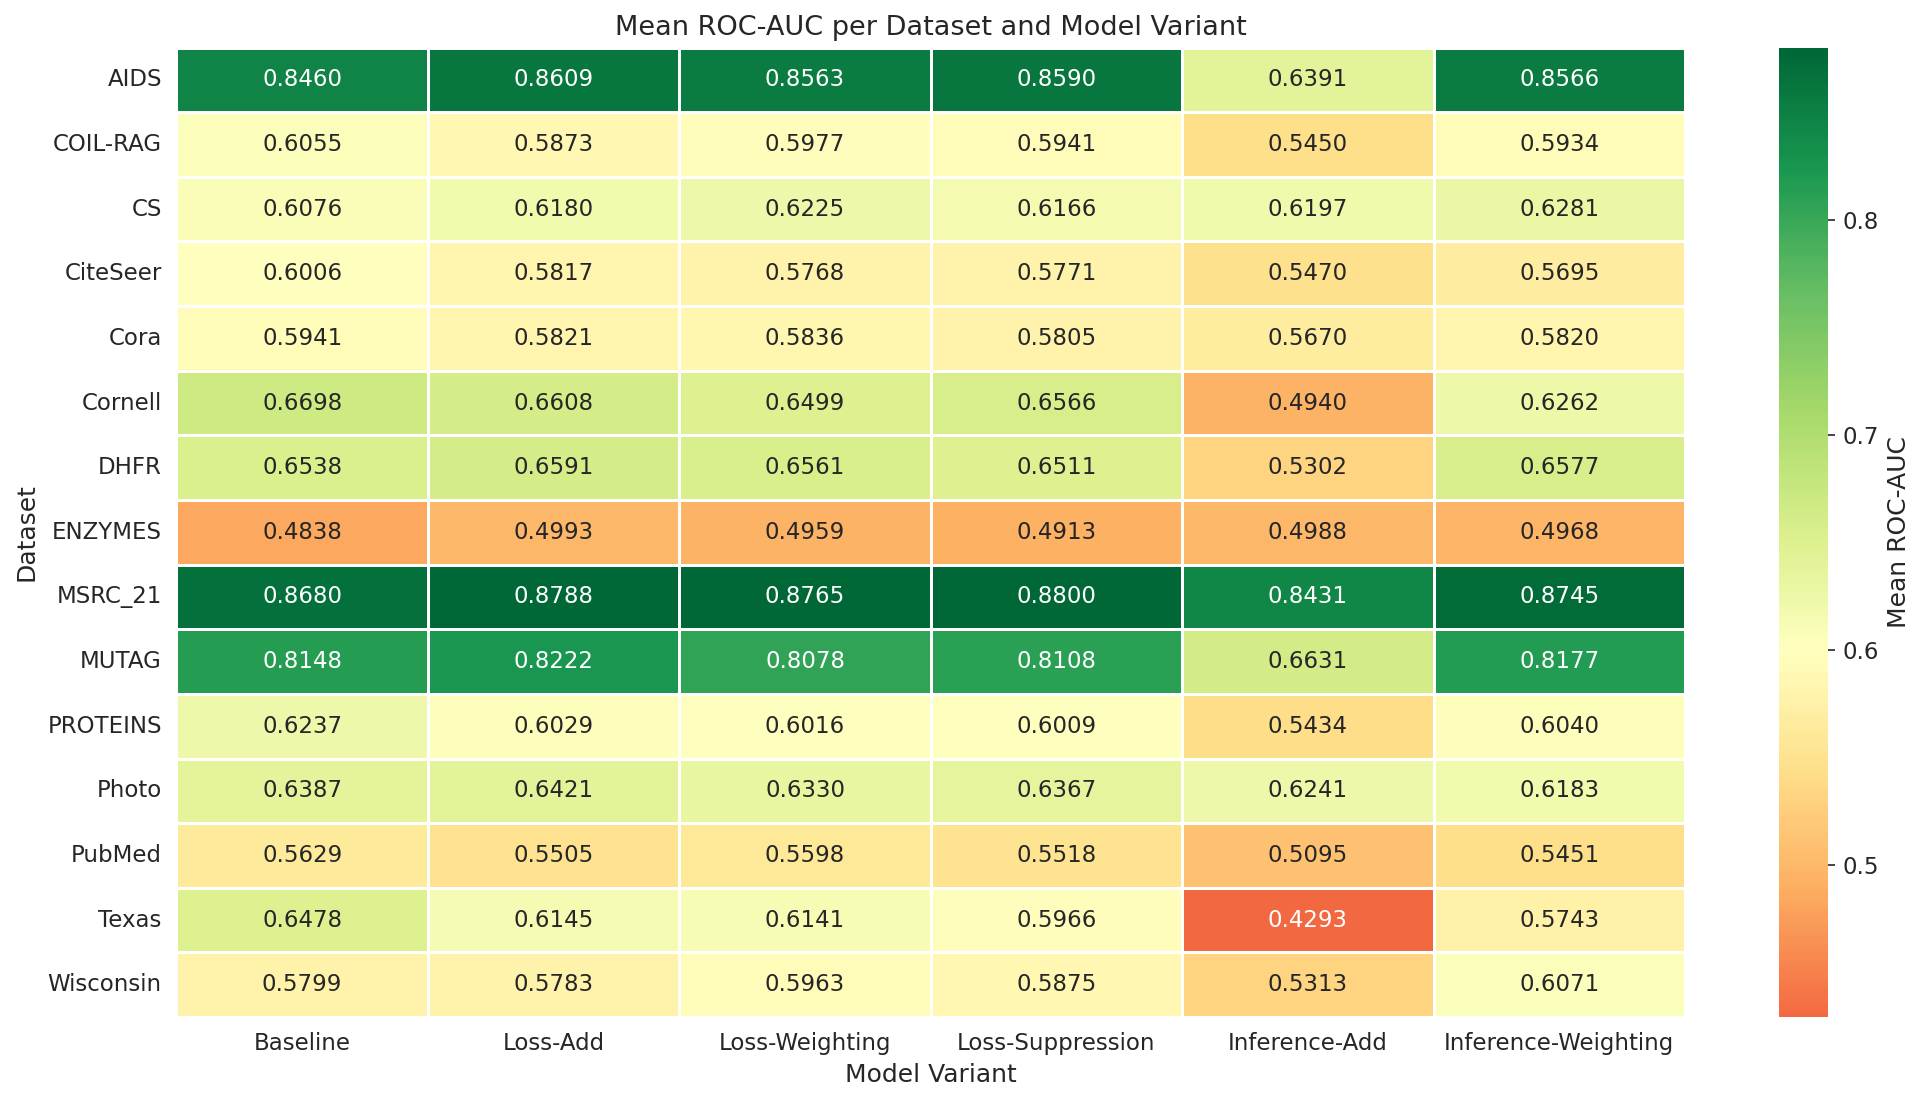
\includegraphics[width=0.75\textwidth]{images/model_ranking_heatmap.png}
        \caption{Mean ROC-AUC per dataset and model variant}
    \end{figure}

    \begin{figure}[htpb]
        \centering
        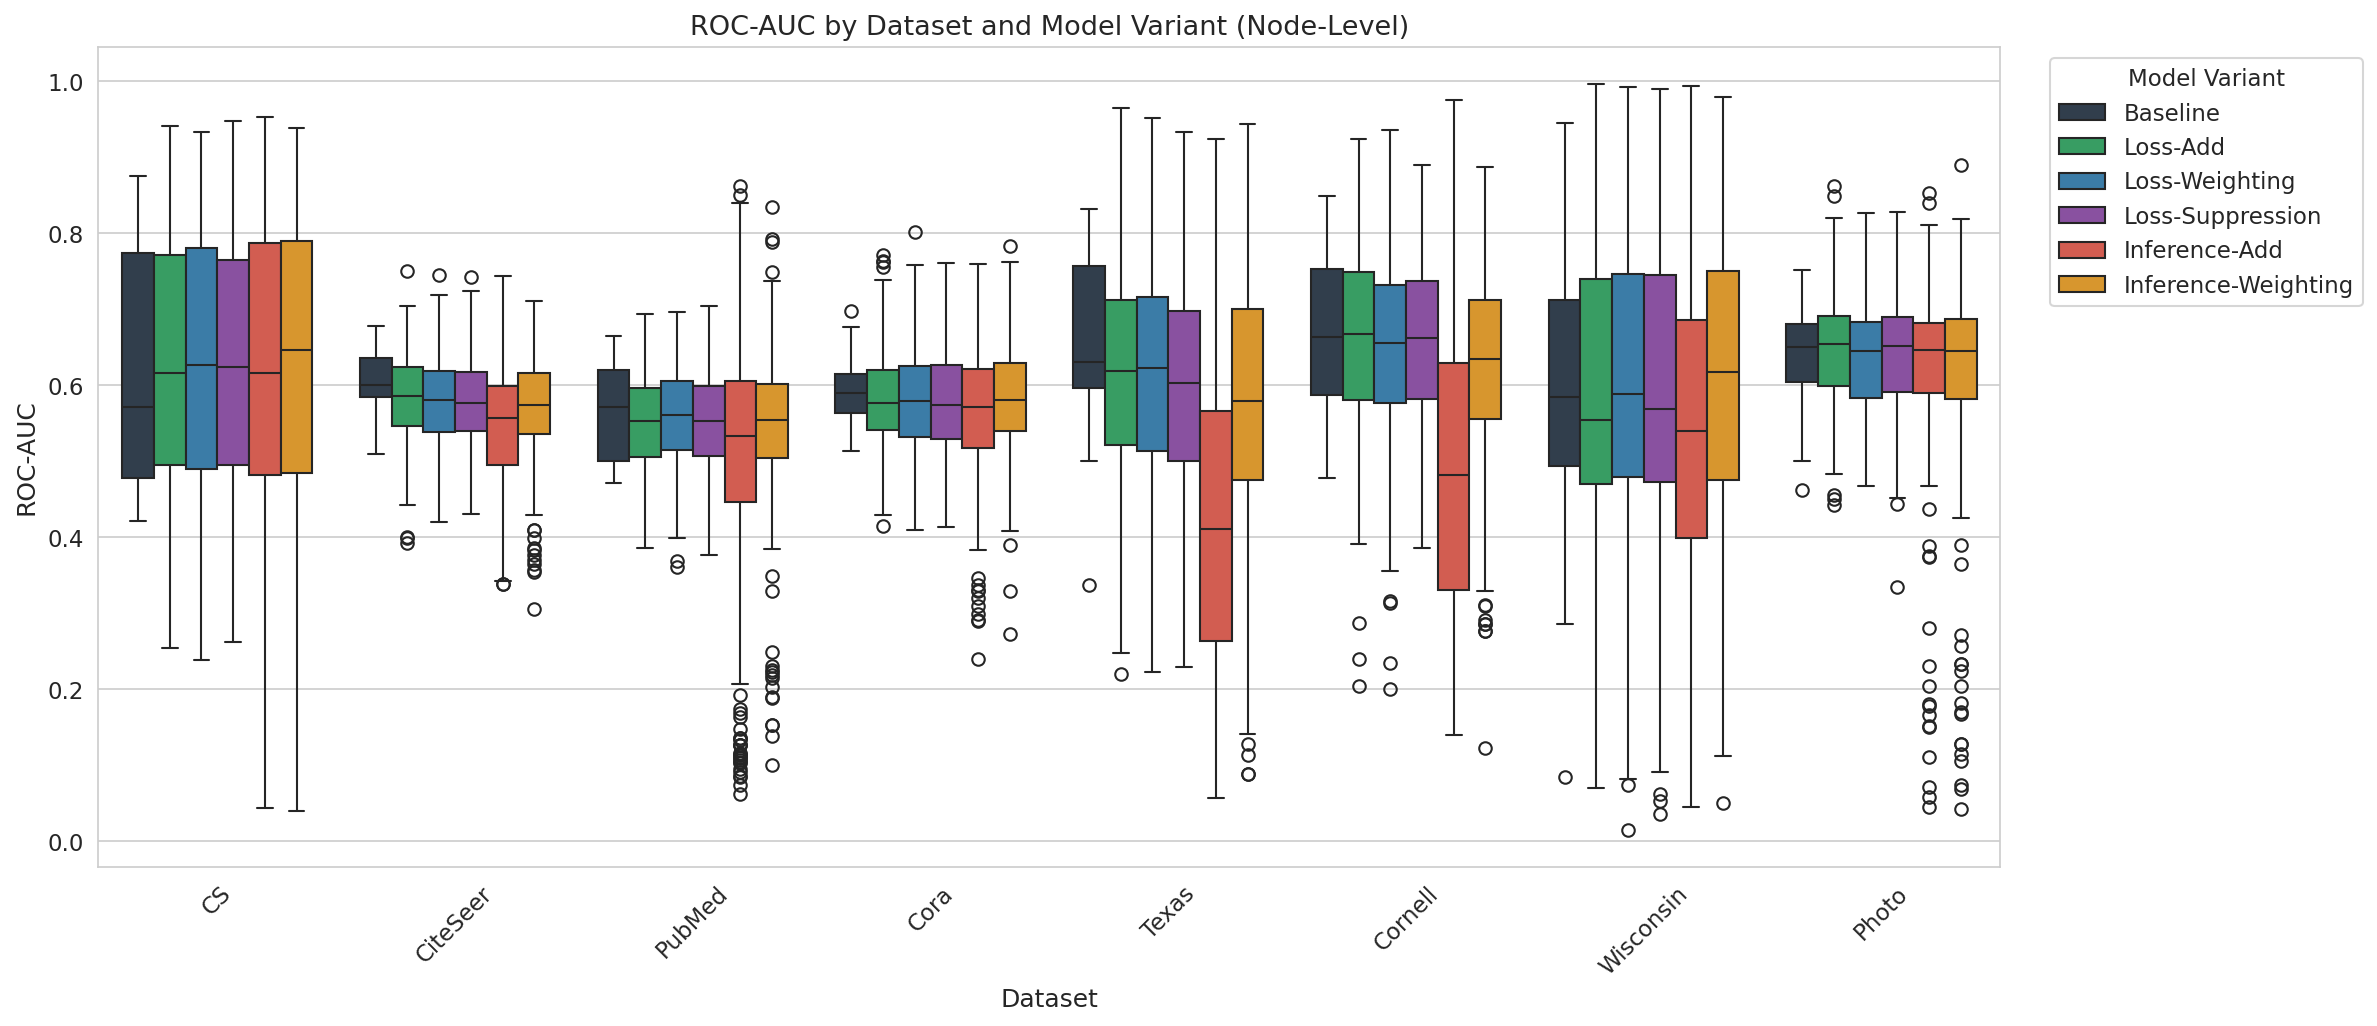
\includegraphics[width=0.75\textwidth]{images/node_roc_auc_boxplot.png}
        \caption{ROC-AUC distribution for node-level prediction}
    \end{figure}
\end{frame}

\begin{frame}{Overall Model Comparison: Statistical Tests}
    \textbf{Mann-Whitney U tests vs.\ baseline:}

    \begin{table}[h]
    \centering
    \begin{tabular}{lcc}
    \toprule
    Model Variant & $p$-value & Significant? \\
    \midrule
    Loss-Add & 0.58 & No \\
    Loss-Weighting & 0.63 & No \\
    Loss-Suppression & 0.40 & No \\
    Inference-Add & $<10^{-10}$ & \textbf{Yes (worse)} \\
    Inference-Weighting & 0.38 & No \\
    \bottomrule
    \end{tabular}
    \end{table}

    \vspace{0.3cm}
    \textbf{Key finding:} Loss-only models preserve baseline performance.
    Inference-Add is significantly worse than all other models.
\end{frame}

\begin{frame}{Loss-Only vs.\ Constraint-Aware Inference}
    \begin{figure}[htpb]
        \centering
        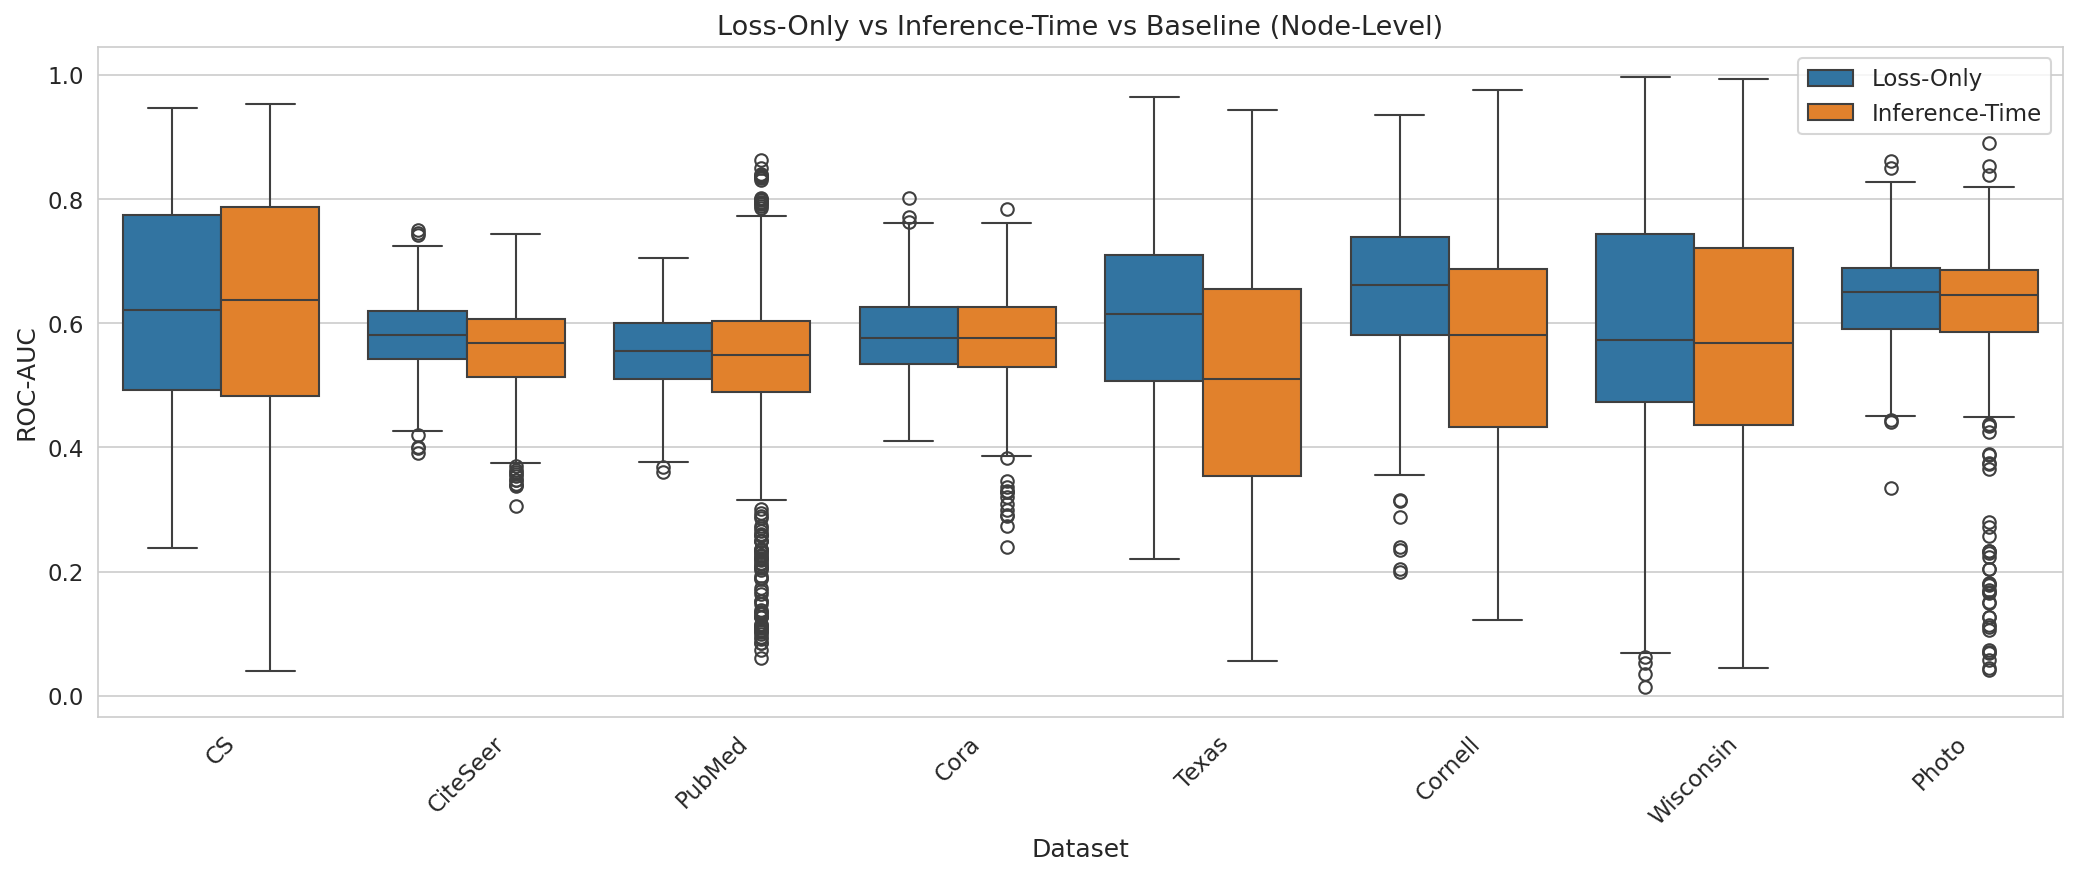
\includegraphics[width=0.8\textwidth]{images/node_loss_vs_inference.png}
        \caption{Loss-only vs.\ constraint-aware inference (node-level)}
    \end{figure}

    \begin{itemize}
        \item \textbf{Loss-only:} not different from baseline ($p = 0.28$ node, $p = 0.92$ graph)
        \item \textbf{Inference-time:} significantly worse ($p = 0.0009$ node, $p = 0.005$ graph)
        \item \textbf{Inference-Add vs.\ Loss-Add:} $p < 10^{-10}$
        \item \textbf{Inference-Weighting vs.\ Loss-Weighting:} $p = 0.27$ (not significant)
    \end{itemize}
\end{frame}

\begin{frame}{Constraint Strength ($\lambda$) Sensitivity}
    \begin{figure}[htpb]
        \centering
        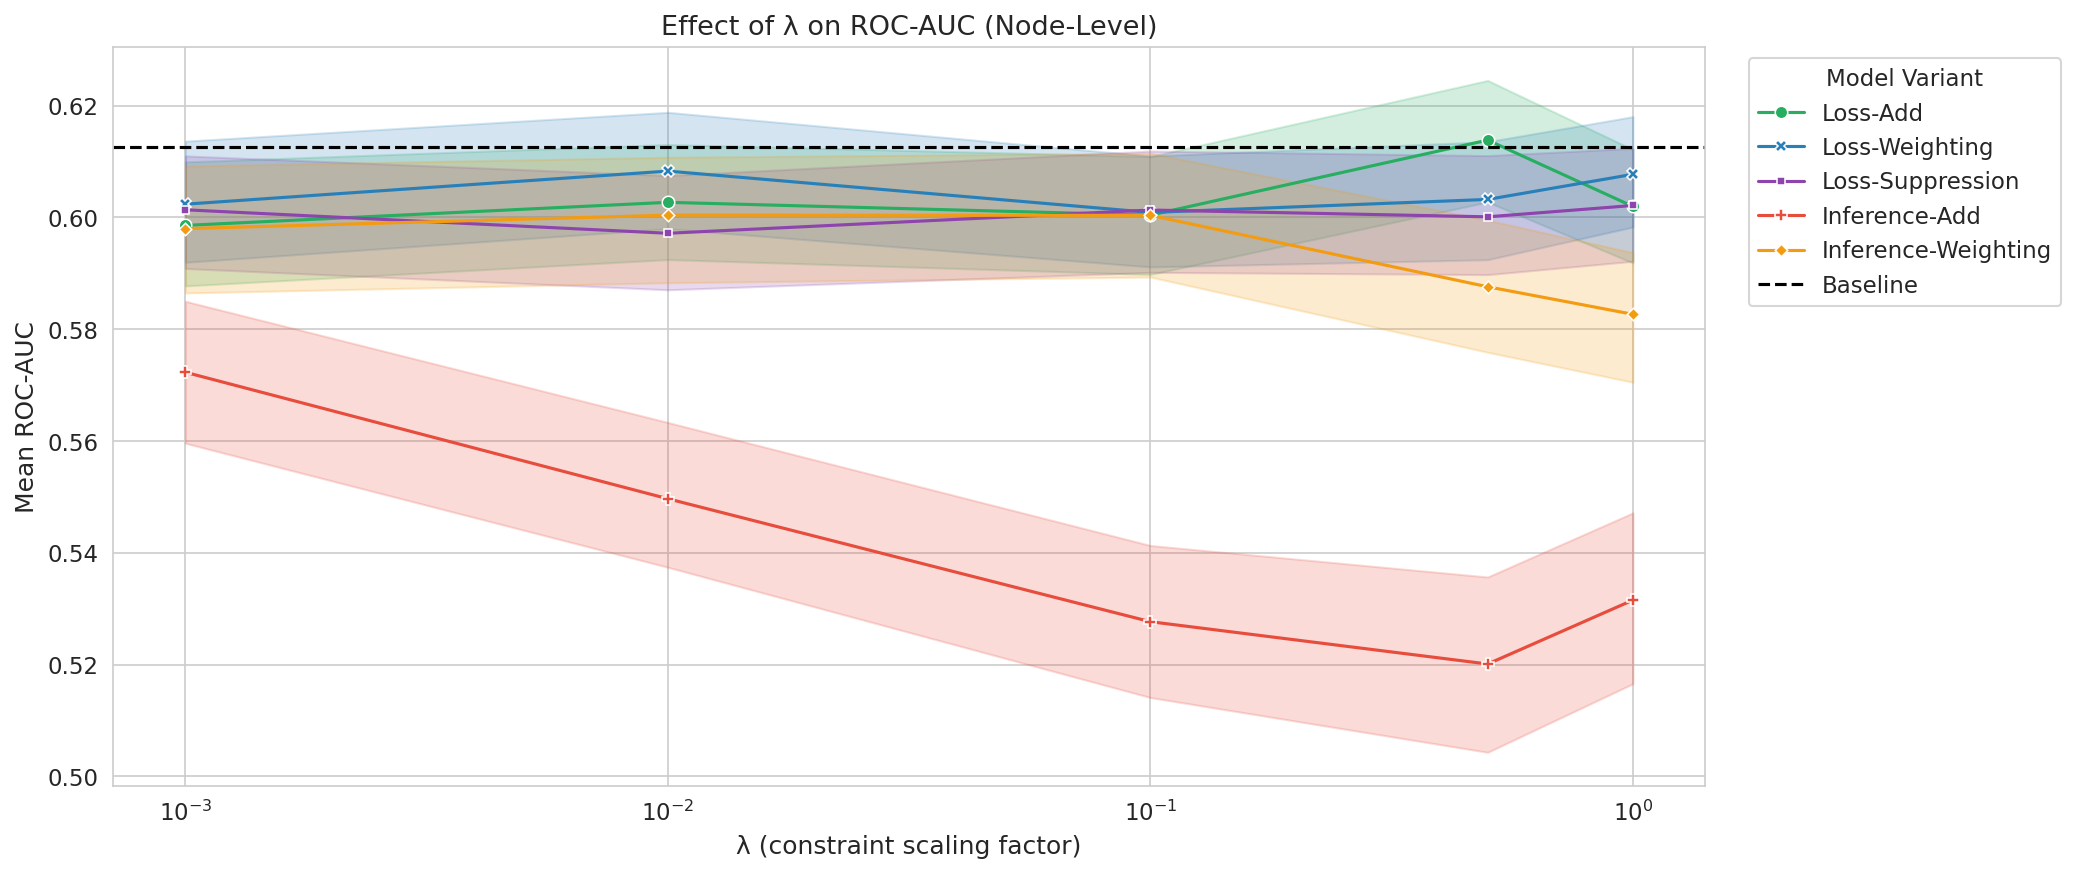
\includegraphics[width=0.8\textwidth]{images/node_lambda_effect.png}
        \caption{ROC-AUC as a function of $\lambda$ (node-level)}
    \end{figure}

    \textbf{Loss-only models:} stable across all $\lambda \in [0.001, 1.0]$
    
    \textbf{Inference models:} highly sensitive --- performance drops sharply with moderate $\lambda$
\end{frame}

\begin{frame}{Handler Comparison}
    \begin{figure}[htpb]
        \centering
        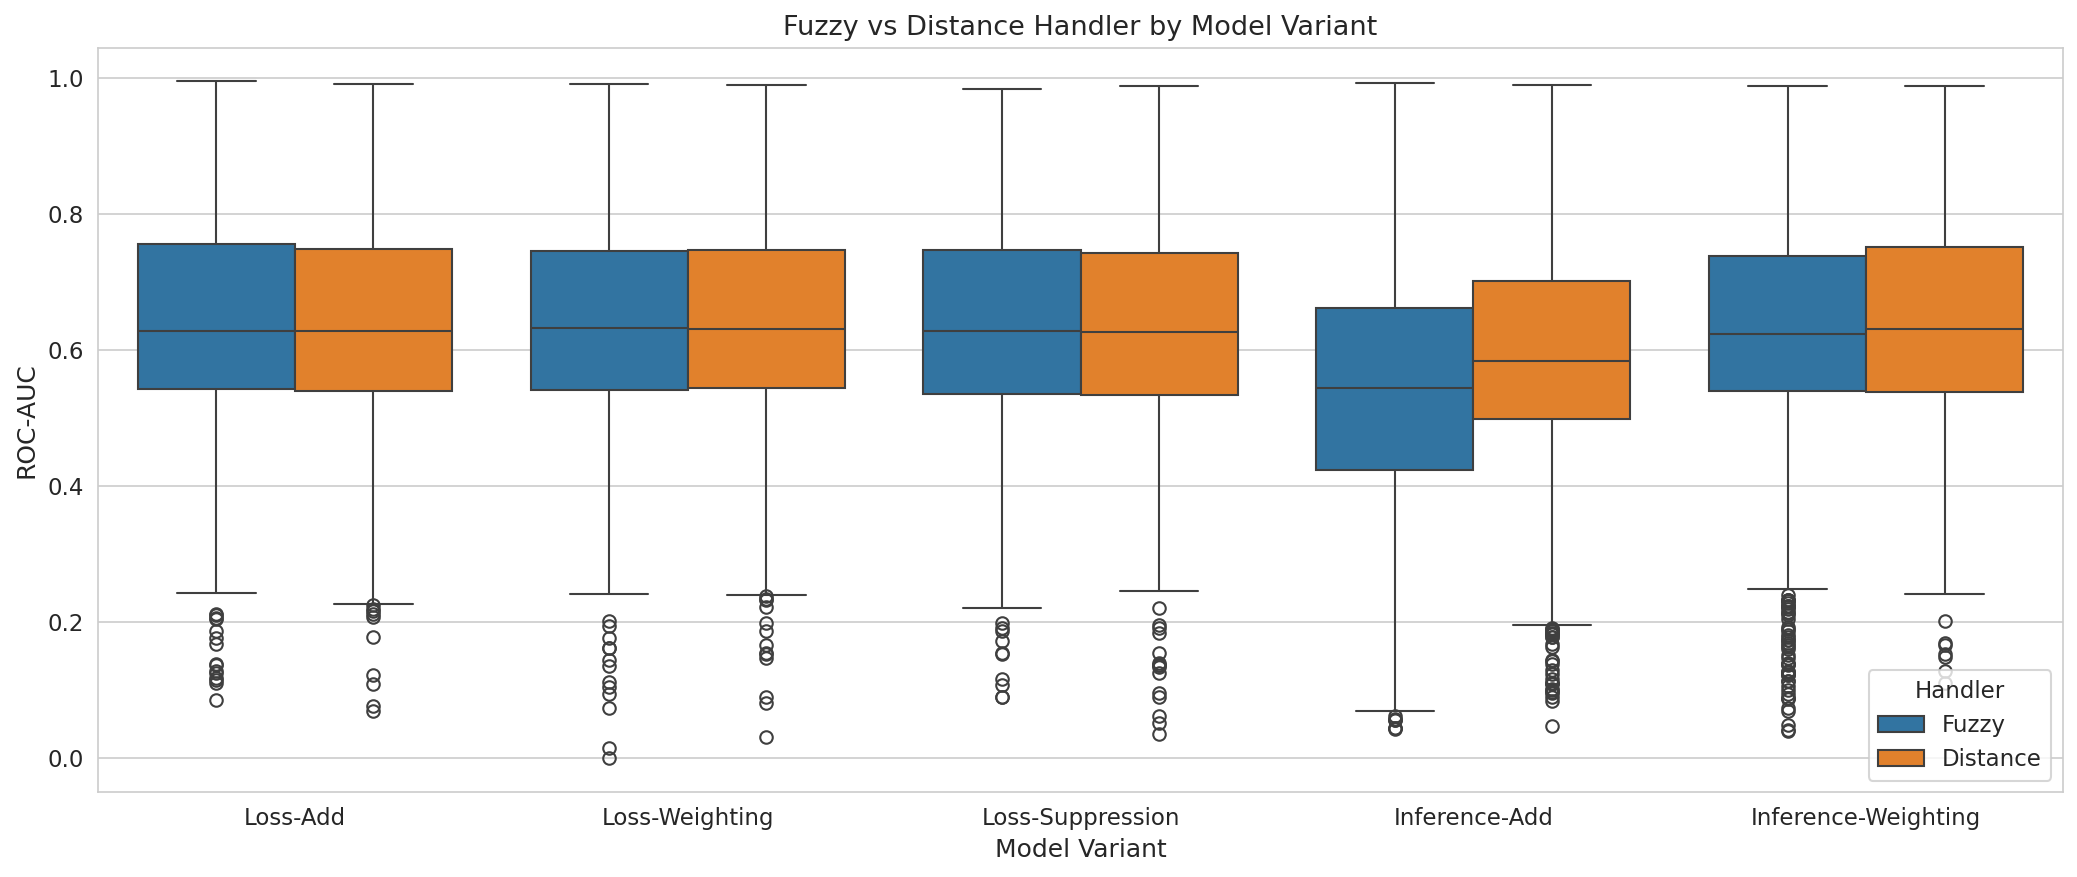
\includegraphics[width=0.8\textwidth]{images/handler_comparison.png}
        \caption{Distance-based vs.\ fuzzy logic handler}
    \end{figure}

    \textbf{Distance-based handler consistently outperforms fuzzy logic} \\
    Mann-Whitney U test: $p = 1.4 \times 10^{-6}$
\end{frame}

\begin{frame}{Best Configurations Per Dataset}
    \textbf{Most striking result: The baseline NEVER achieves the best performance on any dataset.}

    \begin{table}[h]
    \centering
    \small
    \begin{tabular}{l l r c}
    \toprule
    Dataset & Model & ROC-AUC & Handler \\
    \midrule
    CS & Inference-Add & \textbf{0.9529} & Fuzzy \\
    CiteSeer & Loss-Add & \textbf{0.7494} & Distance \\
    Cora & Loss-Weighting & \textbf{0.8013} & Fuzzy \\
    Cornell & Inference-Add & \textbf{0.9753} & Distance \\
    Photo & Inference-Weighting & \textbf{0.8897} & Distance \\
    PubMed & Inference-Add & \textbf{0.8624} & Distance \\
    Texas & Loss-Add & \textbf{0.9645} & Distance \\
    Wisconsin & Loss-Add & \textbf{0.9958} & Fuzzy \\
    \bottomrule
    \end{tabular}
    \hspace{0.3cm}
    \begin{tabular}{l l r c}
    \toprule
    Dataset & Model & ROC-AUC & Handler \\
    \midrule
    AIDS & Loss-Add & \textbf{0.9845} & Distance \\
    COIL-RAG & Loss-Add & \textbf{0.8373} & Distance \\
    DHFR & Inference-Add & \textbf{0.8309} & Distance \\
    ENZYMES & Loss-Add & \textbf{0.7349} & Distance \\
    MSRC\_21 & Loss-Add & \textbf{0.9916} & Distance \\
    MUTAG & Loss-Suppr. & \textbf{0.9854} & Distance \\
    PROTEINS & Loss-Suppr. & \textbf{0.7730} & Fuzzy \\
    \bottomrule
    \end{tabular}
    \end{table}
\end{frame}

\begin{frame}{Key Findings}
    \textbf{Four principal findings:}

    \begin{enumerate}
        \item \textbf{Loss-only constraint models perform indistinguishably from baseline OCGIN} \\
        (all $p > 0.28$, Mann-Whitney U test)
        \item \textbf{Constraint-aware inference introduces $\lambda$ sensitivity} \\
        Carefully tuned $\lambda$ yields best per-dataset results, but default high $\lambda$ degrades performance
        \item \textbf{Inference-Add is significantly worse than all other models} \\
        ($p < 10^{-10}$), while Inference-Weighting does not differ from baseline ($p = 0.38$)
        \item \textbf{Distance-based handler consistently outperforms fuzzy logic} \\
        ($p = 1.4 \times 10^{-6}$), and \textbf{the best config on EVERY dataset uses a constraint model}
    \end{enumerate}
\end{frame}

\section{Conclusion}

\begin{frame}{Conclusion and Future Work}
    \textbf{Summary:}
    \begin{itemize}
        \item Investigated integration of logical constraints into OCGIN
        \item Developed automatic constraint generation pipeline from decision trees
        \item Evaluated 6 model variants across 15 datasets (27,261 trials)
        \item Demonstrated that constraint models can substantially outperform baselines with proper tuning
    \end{itemize}

    \textbf{Future Work:}
    \begin{itemize}
        \item Extend constraint generation to Logic Gate Networks for binary/categorical features
        \item Investigate margin-aware scoring (distance-based handler) further
        \item Adaptive $\lambda$ scheduling or learned constraint weighting
        \item Evaluate on larger and more diverse graph datasets
    \end{itemize}
\end{frame}

\begin{frame}{}
    \centering
    \Large Thank you for your attention!
\end{frame}

\begin{frame}[allowframebreaks]{References}
\printbibliography
\end{frame}

\end{document}
